\chapter[Guidelines]{Guidelines{\color{gray}\,---\,For reference only}}
\section{Sydney 2019}

\begin{itemize}[nosep]
	\item Directional antennas will be used on each arena
	\item Each league will have a separate SSID, on non-conflicting channels
	\begin{itemize}[nosep]
		\item OPL: \texttt{AtHomeOPL}
		\item DSPL: \texttt{AtHomeDSPL}
		\item SSPL: \texttt{AtHomeSSPL}
	\end{itemize}
	\item Each team will have a separate vLAN
	\item Devices will be registered to the vLAN by MAC address, including:
	\begin{itemize}[nosep]
		\item Robots
		\item Laptops
		\item External devices
		\item Non-registered devices will be prevented from connecting to the competition network
	\end{itemize}
	\item No practice network (as some robots are difficult to re-configure)
	\item Network providers will
	\begin{itemize}[nosep]
		\item Monitor network traffic
		\item Identify rouge devices and teams
		\item Register devices to VLANs
	\end{itemize}

\section{Nagoya 2017}
\begin{figure}[H]
	% 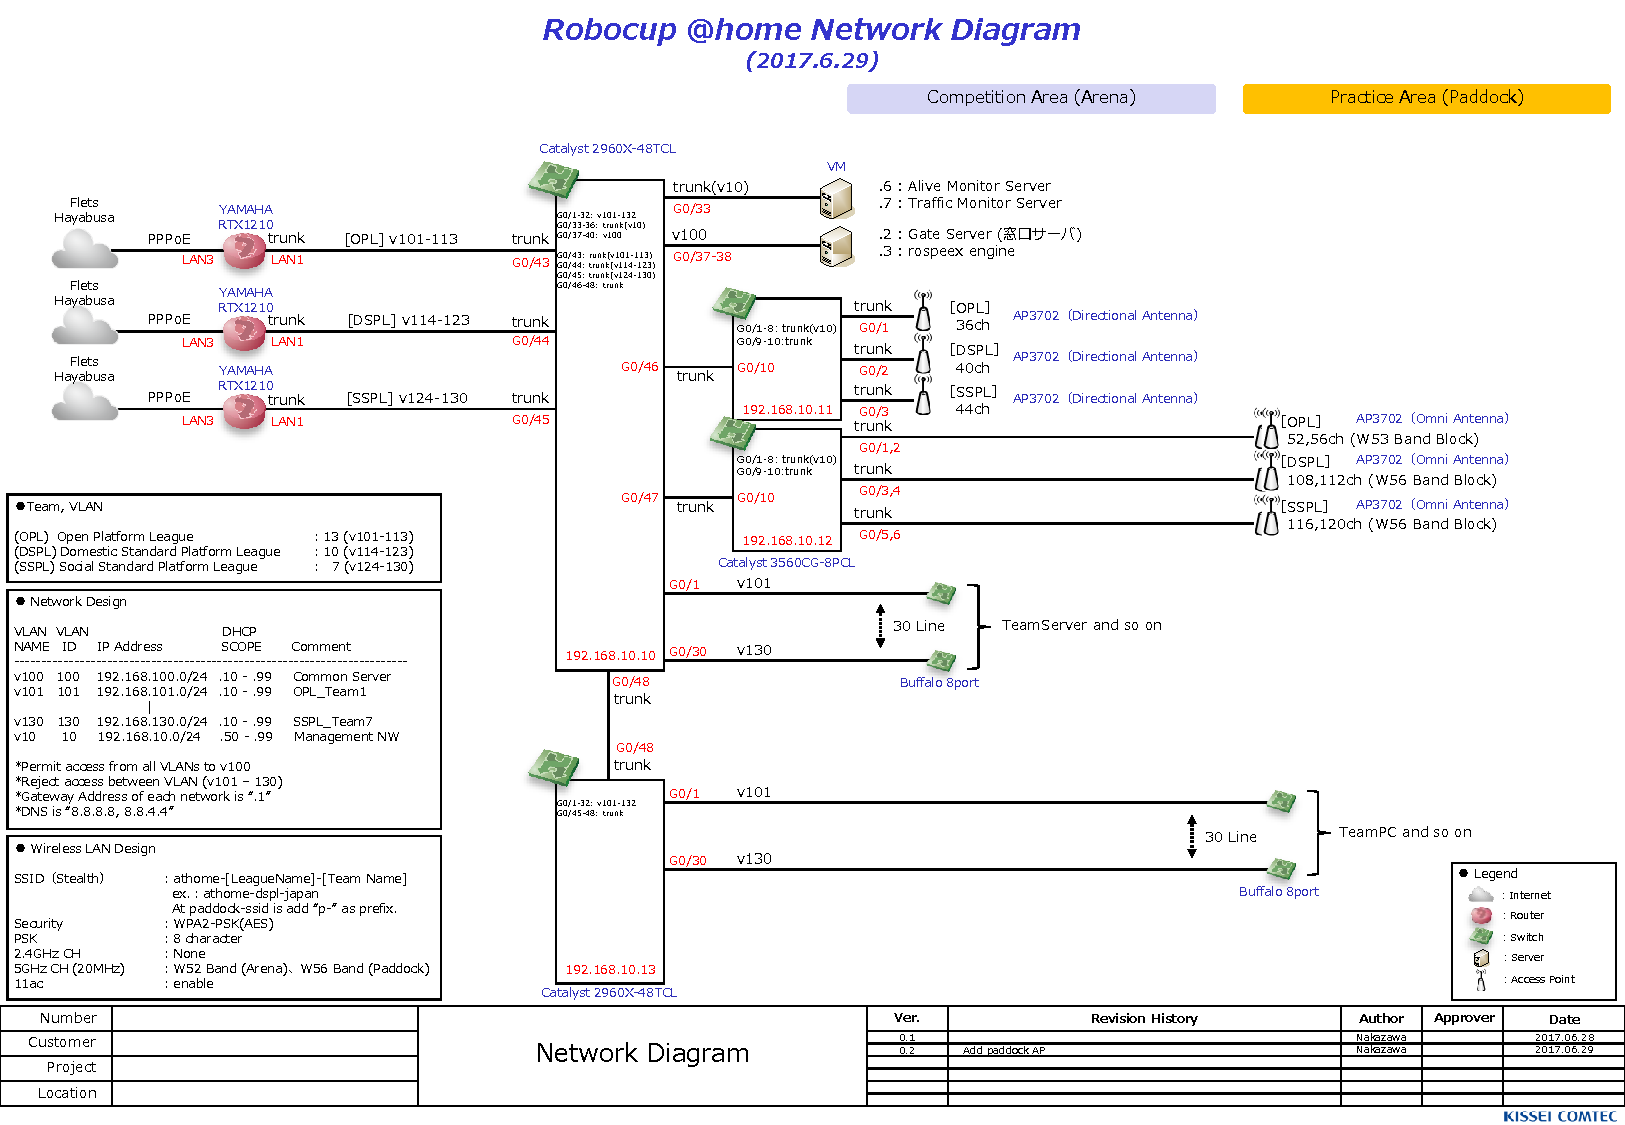
\includegraphics[rotate=90,width=\columnwidth]{images/nago2017_network.pdf}
	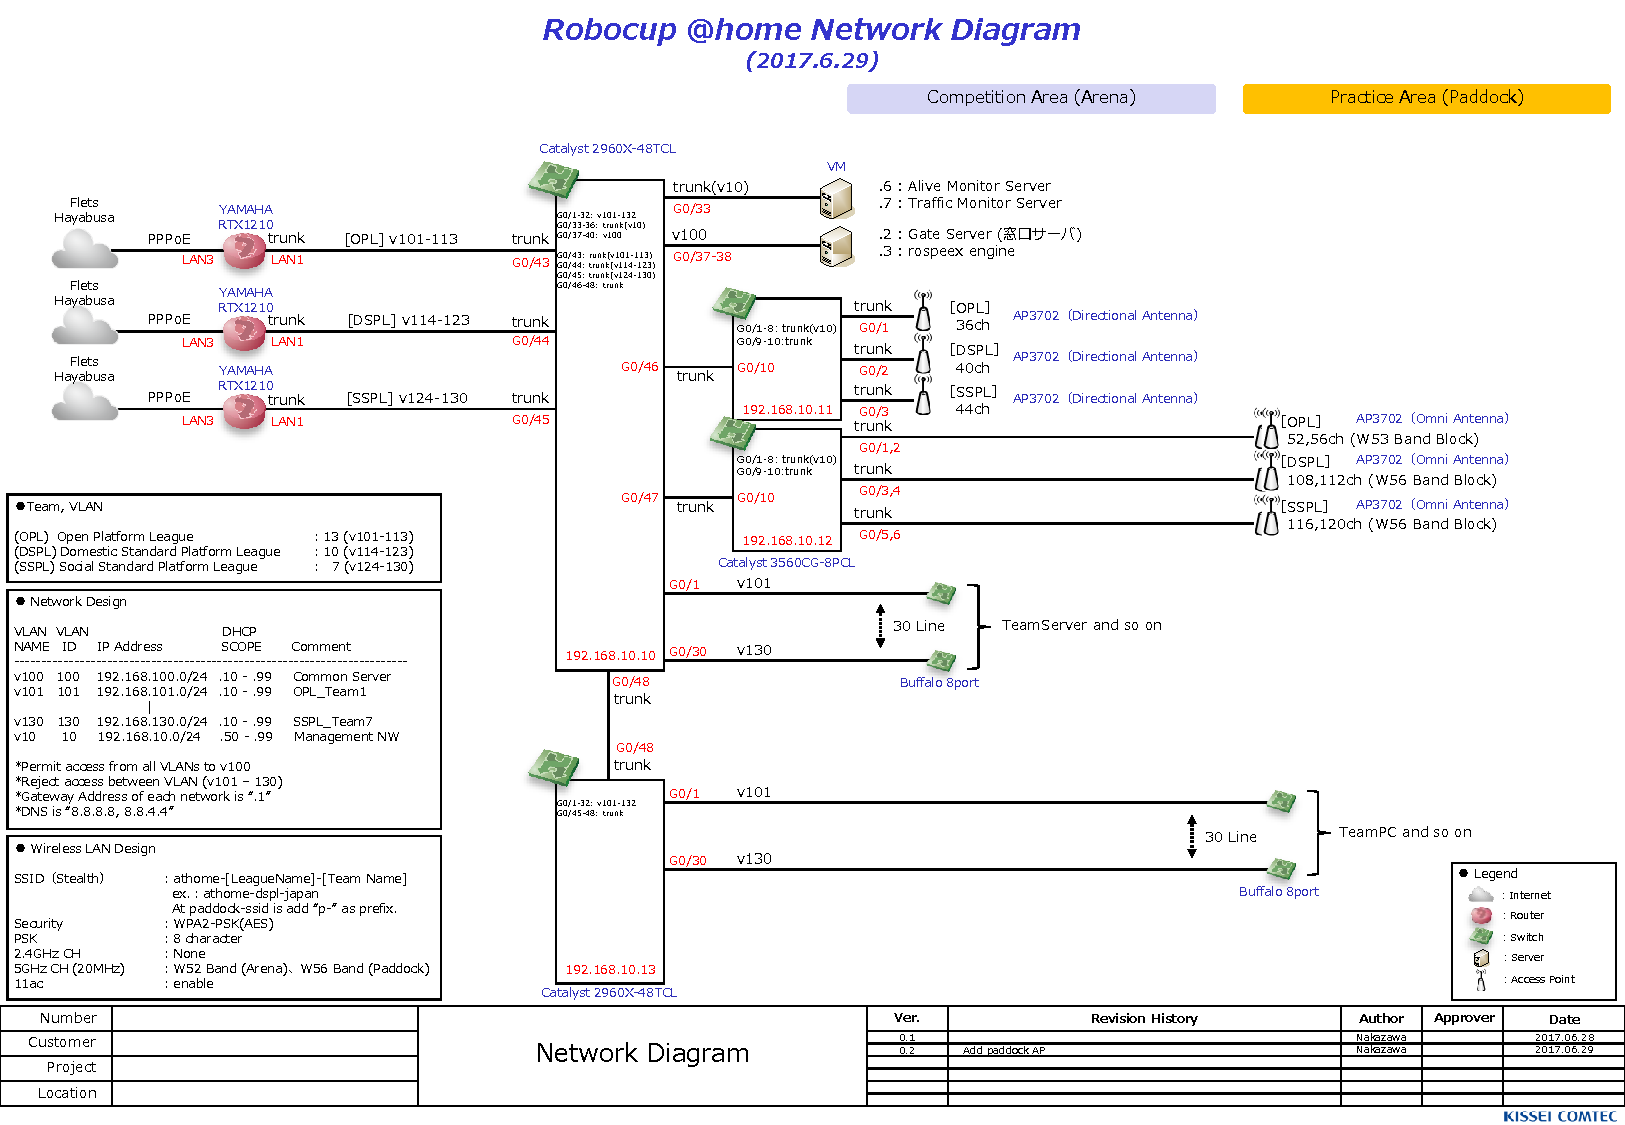
\includegraphics[width=\columnwidth]{images/nago2017_network.pdf}
\end{figure}

\end{itemize}
